%\documentclass{vgtc}                          % final (conference style)
\documentclass[review]{vgtc}                 % review
%\documentclass[widereview]{vgtc}             % wide-spaced review
%\documentclass[preprint]{vgtc}               % preprint
%\documentclass[electronic]{vgtc}             % electronic version


\usepackage{mathptmx}
\usepackage{graphicx}
\usepackage{times}
\usepackage{comment}
\usepackage{caption}
\usepackage{subcaption}
\usepackage{amsmath}
\usepackage{amssymb}
\usepackage{verbatim}
\newenvironment{tightItemize}{
\begin{itemize}
        \setlength{\itemsep}{1pt}
        \setlength{\parskip}{0pt}
        \setlength{\parsep}{0pt}
}{\end{itemize}
}
\usepackage{color}
\newcommand{\fix}[1]{\textcolor{red}{#1}} %Put words in Red
\usepackage[normalem]{ulem} % for cross out words
\usepackage{url}

\onlineid{156}

%% declare the category of your paper, only shown in review mode
\vgtccategory{Research}

%% allow for this line if you want the electronic option to work properly
\vgtcinsertpkg


\title{Preliminary Tests of SPIHT and SPECK Encoders on Scientific Data Sets}


%% Abstract section.
\abstract{
SPIHT and SPECK encoders were originally developed by the image processing community.
%
They provide high image compression ratios while keep the distortions low.
%
We investigate the application of SPIHT and SPECK on scientific data sets 
in this document.
} % end of abstract


%%%%%%%%%%%%%%%%%%%%%%%%%%%%%%%%%%%%%%%%%%%%%%%%%%%%%%%%%%%%%%%%
%%%%%%%%%%%%%%%%%%%%%% START OF THE PAPER %%%%%%%%%%%%%%%%%%%%%%
%%%%%%%%%%%%%%%%%%%%%%%%%%%%%%%%%%%%%%%%%%%%%%%%%%%%%%%%%%%%%%%%%

\begin{document}

\firstsection{Introduction}

\maketitle

\label{sec:intro}
%
SPIHT~\cite{said1996new} and SPECK~\cite{pearlman2004efficient} 
were originally proposed as 2D image encoders.
%
They aim to achieve high image compression ratios while introduce 
a minimal amount of distortion.
%
Empirically, SPIHT, SPECK, and JPEG~2000~\cite{pearlman2004efficient}
share similar \textit{computational complexity} and \textit{accuracy}
on images.


Researchers later extended SPIHT and SPECK to encode three-dimensional
data~\cite{kim1997embedded, tang2006three}. 
%
In this document, we report results from our tests of 
SPIHT and SPECK on 3D scientific data sets.


\section{Study Overview}
%
Our study evaluates the reconstruction accuracy of SPIHT and SPECK
on various data sets. 
%
We compare results from SPIHT and SPECK with two other compression techniques:
1) Discrete Wavelet Transform (DWT), 
and 2) simple truncation that casts a double-precision
floating point number to single-precision.
%
More specifically, 
we operate on single-precision floating point numbers
when comparing with DWT, and on double-precision 
floating point numbers when comparing with truncation.
%
The implementation of SPIHT and SPECK are from QccPack~\cite{fowler2000qccpack},
and the DWT implementations are from VAPOR~\cite{clyne2007interactive}.


DWTs can use different wavelet kernels to perform wavelet transforms,
and each wavelet kernel has its unique characteristics.
%
We specifically choose the CDF~9/7 kernel in this study, since research by
Li~et~al.~\cite{li2015evaluating}
has shown that the CDF~9/7 kernel has most accuracy when compressing 
scientific data sets with similar properties.
%
%As a result, all the use of ``wavelets" and ``DWTs" in the following text
%refers to DWTs with CDF~9/7 wavelet kernel.


We note that the SPIHT and SPECK encoders also involve wavelet transforms
as a subroutine (the complete pipeline is wavelet transform 
$\rightarrow$ quantization $\rightarrow$ SPIHT or SPECK encoding).
%
Multiple wavelet kernels can apply in this subroutine as well.
%
To make a fair comparison, we keep using the CDF~9/7 kernel in 
this subroutine of SPIHT and SPECK.
%
Finally, the quantization subroutine uses the default settings
from QccPack.


Our evaluation criteria are Root Mean Square Error (RMSE) and
maximum point-wise difference (LMax). 
%
RMSE provides an averaged error evaluation and LMax provides the
worst case bound.


\section{Encoders vs. Wavelets}
\label{sec:encoders_wavelets}
%
In this section, we compare the two encoders, SPIHT and SPECK, 
with discrete wavelet transform.
%
Our evaluation compares reconstructed data with the raw data, and 
calculates the RMSE and LMax on each compressed form.
%
The compression ratios are: 4:1, 8:1, 16:1, and 32:1.
%
We use three $512^3$ data sets, all from a turbulent-flow simulation:
the X component of velocity (VX), the X component of vorticity (WX), and enstrophy.
%
Figure~\ref{fig:rmse_fig1} and \ref{fig:lmax_fig2} show the RMSE and LMax evaluations respectively.

\begin{figure}
  \centering
    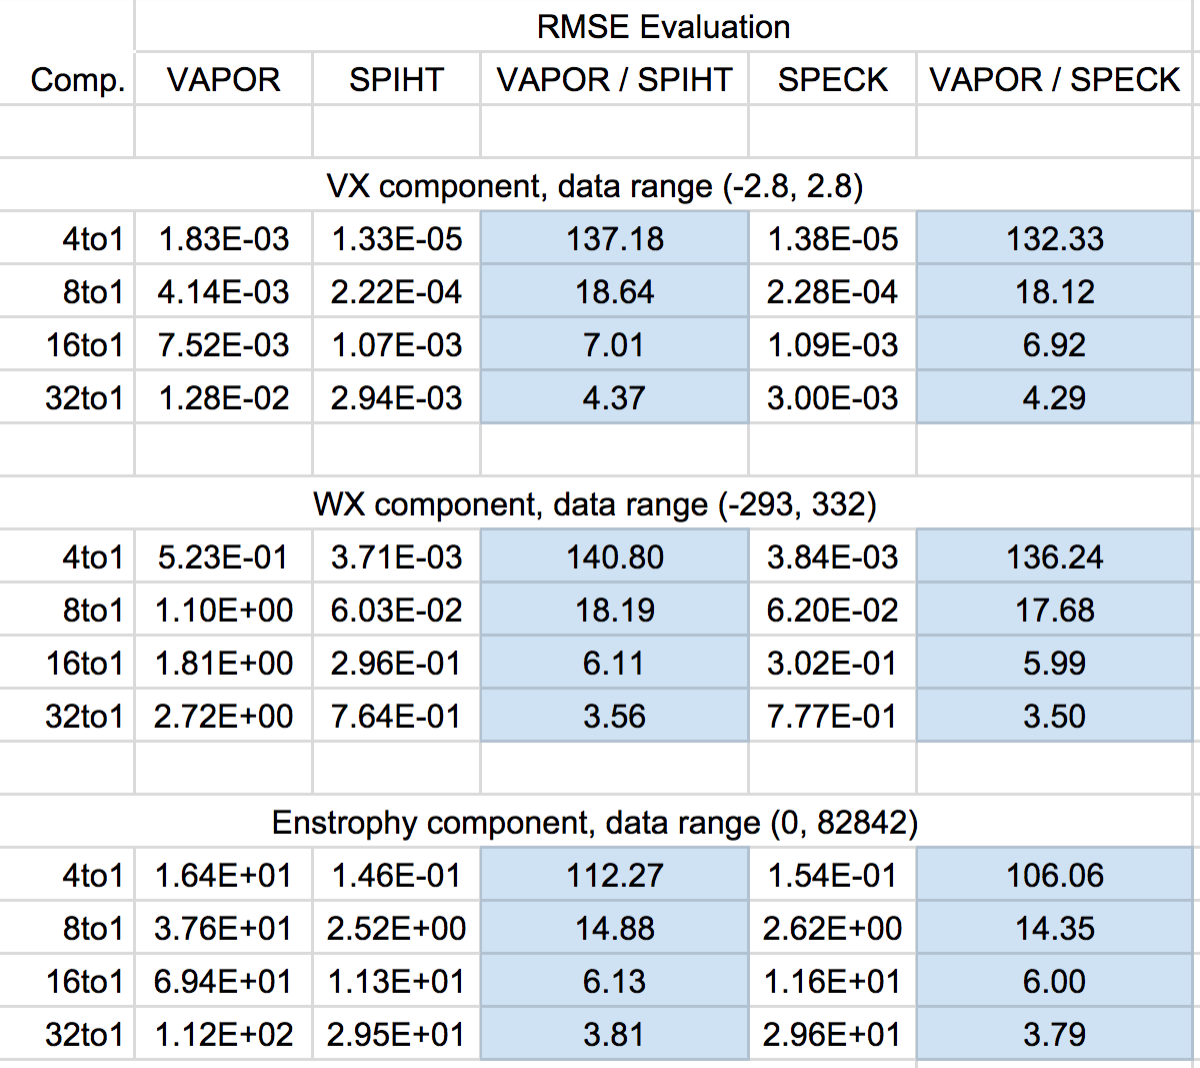
\includegraphics[width=1\columnwidth]{figs/rmse_fig1.png}
  \caption{
RMSE of three data sets, using various compression settings.
%
The three compression techniques are wavelets from VAPOR, 
SPIHT, and SPECK.
%
The improvements of SPIHT and SPECK against VAPOR 
are shown comparatively in blue background.
}
  \label{fig:rmse_fig1}
\end{figure}

\begin{figure}
  \centering
    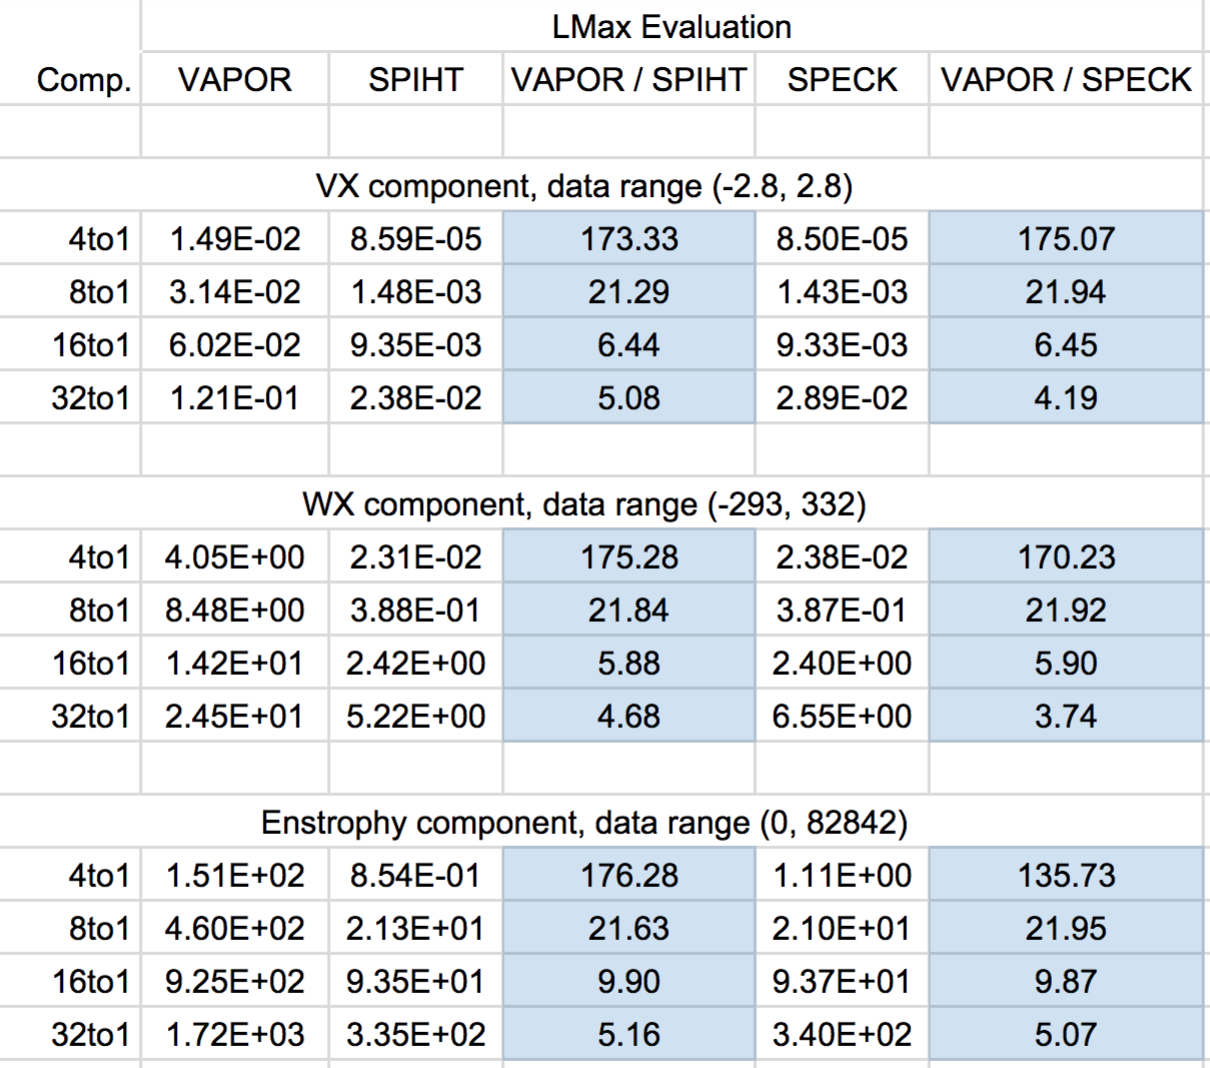
\includegraphics[width=1\columnwidth]{figs/lmax_fig2.png}
  \caption{
LMax of three data sets, using various compression settings.
%
The three compression techniques are wavelets from VAPOR, 
SPIHT, and SPECK.
%
The improvements of SPIHT and SPECK against VAPOR 
are shown comparatively in blue background.
}
  \label{fig:lmax_fig2}
\end{figure}

Both RMSE and LMax evaluations show more accurate results from
SPIHT and SPECK over wavelets. 
%
At the same time, the two encoders, 
SPIHT and SPECK, exhibit similar results.
%
The advantage of SPIHT and SPECK varies on compression ratios:
they are two orders of magnitude better on 4:1, 
but less than one order of magnitude better on 16:1 and 32:1.
%
It is worth keep investigating what are the scenarios to apply 
the two encoders with most gain in accuracy.

This test also shows how the data range affects accuracy.
%
Our narrowest data range is 5.6 and widest is 82842.
%
Interestingly, these three data sets show similar error rates 
at each compression level.
%
This is a little counter-intuitive to us because the quantization step in
SPIHT and SPECK is expected to introduce larger errors when the data range 
is wide.
%
It is worth keep investigating the effects of data range when using
SPIHT and SPECK.


\section{Encoders vs. Truncation}
%
In this section, SPIHT and SPECK encode and decode 
double-precision floating point numbers.
%
Truncation casts a double-precision number to single-precision
(this is widely used when saving the simulation results onto disk).
%
From the standpoint of compression, truncation achieves a compression ratio
of 2:1.
%
Finally, we always use the raw data in double-precision as the baseline to 
compare the compressed data.


\begin{figure}
  \centering
    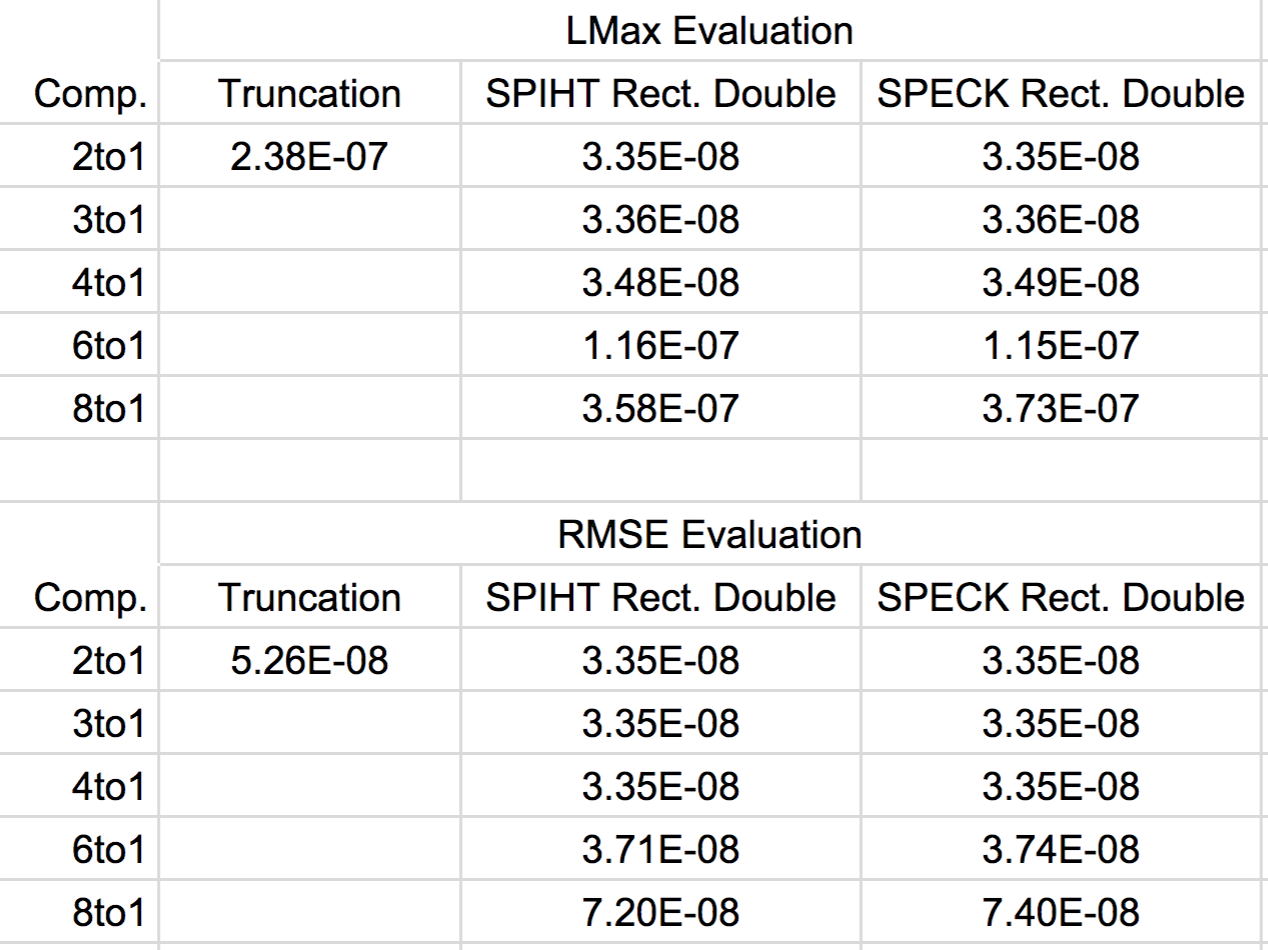
\includegraphics[width=0.9\columnwidth]{figs/truncation_fig3.png}
  \caption{
LMax and RMSE errors of truncation, SPIHT, and SPECK encoders.
%
Note that truncation only supports 2:1 compression ratio.
%
The test data set is Marschner-Lobb data set at $256^3$ resolution,
ranging from 7.6E-6 to 1.
}
  \label{fig:truncation_fig3}
\end{figure}


Figure~\ref{fig:truncation_fig3} shows the comparison between the two encoders 
and truncation using the Marschner-Lobb data set.
%
This data set has a resolution of $256^3$ and data range (7.6E-6, 1).
%
The results show that both SPIHT and SPECK introduce less error at the 2:1 level, 
the compression ratio that truncation achieves.
%
Also, the two encoders reach comparable error rates with truncation
at more aggressive compression ratios, between 6:1 and 8:1 in this case.
%
We are especially pleased to see that SPIHT and SPECK have superior performance
than truncation even in terms of the LMax metric.


In a second test, we compare the SPECK encoder with truncation using
a climate data set.
%
This data set contains both 2D and 3D variables, and we especially tested
157 3D variables.
%
These 3D variables have dimensions $60\times384\times320$.
%
This data set is also special in that it has missing values
(e.g. some vertices in the mesh are not valid).
%
Since SPECK encoder is not able to handle missing values,
we take a preprocessing step to replace all the missing values in a variable 
with the average of all the valid values.
%
This preprocessing step was only for SPECK to encode and decode correctly, 
and we calculated RMSE and LMax only on the valid data points.

We group test results from all 157 variables into four categories.
%
Each variable falls into one of the four categories 
based on how many times SPECK performs better than truncation:
1) no improvement ($< 1\times$ imprv.),
2) less than ten times improvement ($< 10\times$ imprv.),
3) less than a hundred times improvement ($< 100\times$ imprv.), 
and 4) equal or greater than a hundred times improvement
($>= 100 \times$ imprv.).
%
Figure~\ref{fig:histogram} summarizes these four categories.
%
Still, we consider the results from the LMax metric most important
and they show significant benefit of using SPECK instead of truncation.

\begin{figure}
  \centering
    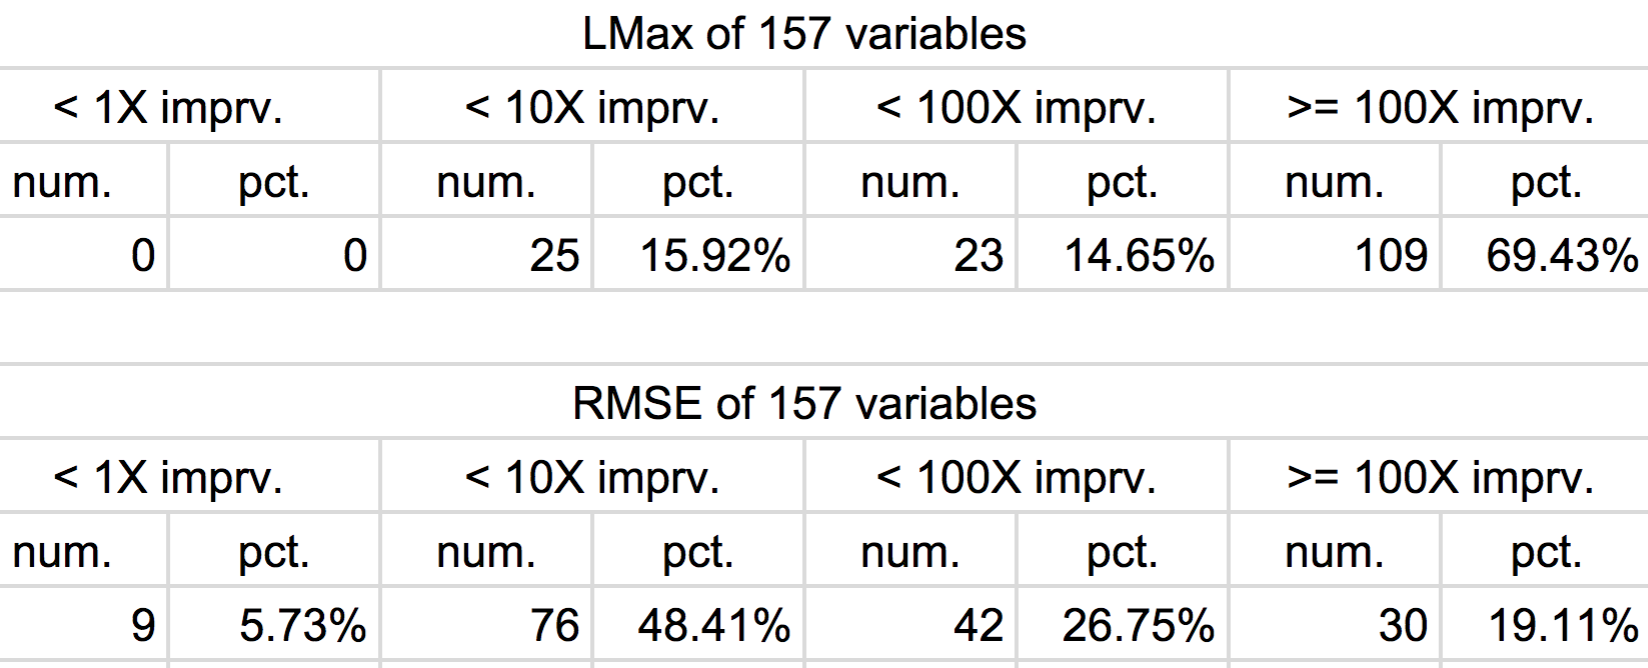
\includegraphics[width=1\columnwidth]{figs/histogram.png}
  \caption{
The number and percentage of variables in each of the four categories.
%
Each category has variables that gain certain amount of improvement by
using SPECK over truncation.
%
The upper figure shows results calculated based on LMax error metric,
and the bottom figure shows results calculated based on RMSE error metric.
}
  \label{fig:histogram}
\end{figure}


\section{Calculation Time}
%
The SPECK and SPIHT encoders take significant amount of time to perform
encoding and decoding tasks. 
%
Since truncation takes almost no time to complete, I compared
SPIHT and SPECK with DWT.
%
My simple and preliminary tests show that SPECK takes $13\times$ time to encode,
and $21\times$ time to decode, when both SPECK and DWT run in serial.
%
SPIHT has similar calculation time.


\section{Additional Properties and Limitations}
%
\textbf{Progressive Access.}
%
Both SPIHT and SPECK encode data into bit-streams. 
%
When decoding, any prefix of the bit-stream can be used to reconstruct
the rectilinear mesh, and more incoming bits will contribute to 
more accurate reconstructions.

\textbf{Always Lossy.}
%
SPIHT and SPECK quantize data before encoding,
and de-quantize it after decoding.
%
These steps make SPIHT and SPECK always introduce some error,
even when encoding to a target size that is the same as the raw data.
%
We can also observe it from Figure~\ref{fig:truncation_fig3}:
SPIHT and SPECK have almost the same error with compression ratios
4:1, 3:1, and 2:1.

\textbf{Power-of-two Constraint for SPIHT.}
%
The use of \textit{zerotrees} in SPIHT encoder introduces the constraint that
each dimension of the grid has to be a power of two.
%
SPECK does not have this constraint, because it is not based on zerotrees.
%
More details on this constraint could be found at~\cite{qcc1}.


\section{Conclusion}
%
SPIHT and SPECK are state-of-the-art encoders from the image processing
community, and their use on scientific data just starts.
%
Our preliminary experiments show both pros and cons of these encoders. 
Namely:

Pros:
\begin{tightItemize}
    \item Up to two orders of magnitude more accurate than DWT
          when performing lossy compression.
    \item Use $3\times$ to $4\times$ less space than truncation
          when saving double-precision floating point data to single-precision.
    \item Support progressive data access. 
\end{tightItemize}

Cons:
\begin{tightItemize}
    \item Computational intensive. Could be $20\times$ slower than DWT.
    \item Always introduce error. Only suit for lossy compression use cases.
    \item SPIHT requires data dimensions be powers of two.
\end{tightItemize}


\bibliographystyle{abbrv}
%%use following if all content of bibtex file should be shown
%\nocite{*}
\bibliography{template}
\end{document}
